\documentclass[]{article}
\usepackage[]{graphicx}
\title{Power Outage Poller: Purpose and Progress}
\author{Jacob Pavelka}

\begin{document}
\maketitle

The purpose of this project is to gather all information available from our communicating devices and external sources to better inform decision-making processes.

Currently, this project's main focus is gathering power outage data to combat severe weather events. To do this, we use Selenium's Webdriver to scrape information about electricity meter status from Oncor's website. We then use that to determine whether communication failures between our management facility and the traffic signal are caused by a lack of power. This helps us diagnose issues with our traffic signals. However, in our projects current state, the information is gathered from the web but remains in an offline database. We wish to integrate this data with our current GIS data, displaying power outage information on MAXVIEW through ArcGIS Online (AGO) and enhancing our response to weather events.

We require your aid in setting up a mechanism to transfer our separately generated database to AGO on a regular basis, then have AGO synchronize with MAXVIEW, our Advanced Traffic Management system.

The rest of this document contains details on the current state of our project. As mentioned before, we are using Selenium's Webdriver to scrape power outage data from Oncor's website. This process begins with a list of known "ESI ID", which uniquely mark each power meter that is servicing the city's traffic signals. A typical list of ESI ID's are shown in Figure~\ref{fig:ids}.
\begin{figure}[htbp]
    \centering
    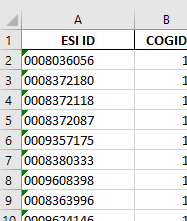
\includegraphics{esi_id.PNG}
    \caption[short]{An example list of ESI IDs}
    \label{fig:ids}
\end{figure}
The Webdriver takes each id from this list, inserts it into the Oncor's web GUI, and then requests information about the meter's status. Interaction with Oncor's webpage is shown in Figure~\ref{fig:oncor_in}. 
\begin{figure}[h]
    \centering
    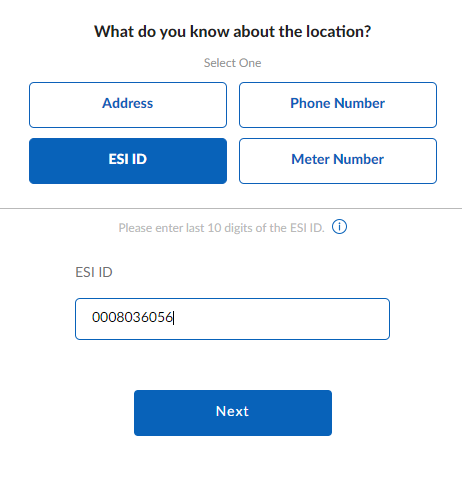
\includegraphics[width=0.6\textwidth]{oncor_esi_in.PNG}
    \caption{GUI interface in which ESI ID's are inputted}
    \label{fig:oncor_in}    
\end{figure}
A new webpage loads based on this process, and it is parsed to update the meters status. A typical webpage that is loaded is shown in Figure~\ref{fig:oncor_out}.
\begin{figure}[h]
    \centering
    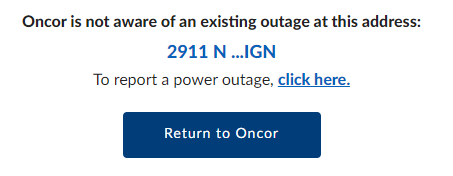
\includegraphics[width=0.6\textwidth]{oncor_status.PNG}
    \caption{Results generated from Oncor's GUI}
    \label{fig:oncor_out}    
\end{figure}
Scraping Oncor's web GUI like this is a lengthy process currently, taking over an hour to update all meters, but we hope to improve this speed later on. In any case, this process can be ran continuously, providing a full update every hour. Currently, the results are stored on a local database. The next task is to upload the results hourly to our interfaces.

\end{document}


Here is a status update on the power outage project:

As we discussed before, the basic functionality of the app works (apart from checking modem failure against controller failure), but it is not operated easily because the users authentication key must be manually entered for the program to work. Even when the users key is entered, the program only works for one hour, so it is not set up to run for long periods of time or automatically.

The authentication system Ericsson is using is the major blockage right now. I thought there might be a way for users to automatically authenticate themselves when they run the program or even automatically authenticate a default user every time the program is ran. However, after investigating it for some time, I do not think this can be easily done. It seems Ericsson never really intended for its end users to be able to implement the sort of tools like the power meter status update tool. Basically, the only way we can access CUT is to go through the webpage first. We have several options moving forward. The first, simplest, and least elegant would be to have a prompt come up every hour when authentication expires and have the user manually apply their user key. A local app/program could do the trick in this case, and the program can still run even when authentication is not available. It would just not be able to get comm failure status. Applying the auth key might be able to be somewhat automated with web scraping, and refresh tokens might be able to be used to be used to increase the authentication length to greater than one hour. Another option we could do is to make a full web app that is exposed and has its own certificates. If this kind of app is developed, the web app might be able to be set up to be directly queried by the CUT API, or we could add its URI to the AAD for redirects and get authentication that way. These are the main options for integrating with CUT. However, If there is some way to create an API user that just needs a username and password for authentication, then that would also make it work much easier as only those credentials would need to be provided and we wouldn't have to go through Azure.

Other solutions are available for long-term status updating apart from using CUT. Each controller can be directly queried for comm failure status, and we have authorization for these queries.